% Template for seminar reports
% Computer Vision Group, Visual Computing Institute, RWTH Aachen University
\documentclass[twoside,a4paper,10pt,DIV=12,BCOR=12mm]{scrartcl}
\usepackage[utf8]{inputenc}    % allows special symbols in LaTeX source code
\usepackage[english]{babel}    % select language of your report (use "ngerman" for German)
\usepackage[T1]{fontenc}       % font encoding, important for umlauts
\usepackage{lmodern}           % lmodern font
\usepackage{xcolor}            % use and define colors for text and images
\usepackage{graphicx}          % include images
\usepackage{booktabs}          % pretty tables
\usepackage{caption}           % captions for figures
\usepackage{subcaption}        % captions for subfigures
\usepackage{url}               % for website links
\usepackage{datetime}          % month on title page
\usepackage{hyperref}          % make references clickable
\usepackage{xspace}            % correct spaces after e.g. "e.g."
\usepackage{tikz}              % custom plots in LaTeX
\usepackage{pgfplots}          % custom function graphs in LaTeX
\usepackage{bm}                % bold math symbols
\usepackage{amsmath}           % additional math environments
\usepackage{amssymb}           % additional math symbols (includes amsfonts)
\usepackage{enumitem}          % change distances for enumerations
\usepackage{listings}          % code
\usepackage{lipsum}            % placeholder text
\usepackage{listings}
\usepackage{color}

\definecolor{dkgreen}{rgb}{0,0.6,0}
\definecolor{gray}{rgb}{0.5,0.5,0.5}
\definecolor{mauve}{rgb}{0.58,0,0.82}

\lstset{frame=tb,
  language=python,
  aboveskip=3mm,
  belowskip=3mm,
  showstringspaces=false,
  columns=flexible,
  basicstyle={\small\ttfamily},
  numbers=none,
  numberstyle=\tiny\color{gray},
  keywordstyle=\color{blue},
  commentstyle=\color{dkgreen},
  stringstyle=\color{mauve},
  breaklines=true,
  breakatwhitespace=true,
  tabsize=3
}

\newdateformat{monthyeardate}{\monthname[\THEMONTH] \THEYEAR}

\setlength{\parindent}{0pt}
\setlength{\parskip}{0pt}
\setlist{nosep}

\makeatletter
\DeclareRobustCommand\onedot{\futurelet\@let@token\@onedot}
\def\@onedot{\ifx\@let@token.\else.\null\fi\xspace}
\def\eg{{e.g}\onedot} \def\Eg{\emph{E.g}\onedot}
\def\ie{{i.e}\onedot} \def\Ie{\emph{I.e}\onedot}
\def\cf{{c.f}\onedot} \def\Cf{\emph{C.f}\onedot}
\def\etc{{etc}\onedot} \def\vs{\emph{vs}\onedot}
\def\wrt{w.r.t\onedot} \def\dof{d.o.f\onedot}
\def\etal{\emph{et al}\onedot}
\makeatother

\overfullrule=1ex

\pgfplotsset{compat=newest}


\tikzset{basic/.style={draw,fill=none,
                       text badly centered,minimum width=3em}}
\tikzset{input/.style={basic,circle,minimum width=3.5em}}
\tikzset{weights/.style={basic,rectangle,minimum width=2em}}
\tikzset{functions/.style={basic,circle, minimum width=3em}}
\newcommand{\addaxes}{\draw (0em,1em) -- (0em,-1em)
                            (-1em,0em) -- (1em,0em);}
\newcommand{\relu}{\draw[line width=1.5pt] (-1em,0) -- (0,0)
                                (0,0) -- (0.75em,0.75em);}
\newcommand{\stepfunc}{\draw[line width=1.5pt] (0.65em,0.65em) -- (0,0.65em) 
                                    -- (0,-0.65em) -- (-0.65em,-0.65em);}


% =========================================================================

\graphicspath{{pictures/}}
\setcounter{secnumdepth}{3}
\setcounter{tocdepth}{3}

% =========================================================================
\begin{document}

% Template for seminar reports
% Seminar Current Topics in Computer Vision and Machine Learning

\begin{titlepage}
\begin{center}
\ 
\vspace{3.5cm}

\textsf{
RWTH Aachen University \\
Faculty of Mathematics, Computer Science and Natural Sciences\\
Chair of Computer Science 13 (Computer Vision) \\
Prof. Dr. Bastian Leibe
}

\rule{\linewidth}{1pt}

\vspace{1.75cm}
\LARGE
\textbf{Proseminar Report}

\vspace{1.7cm}
\huge
Long Short Term Memory

\vspace{3.0cm}
\Large
Leon Benz\\
\large
Matriculation Number: 445034
\vspace{0.25cm}
\Large
Fynn Jansen\\
\large
Matriculation Number: 467964

\vspace{0.5cm}
\monthyeardate\today

\vspace{1.05cm}
\rule{\linewidth}{1pt}

\vspace{0.5cm}
\textsf{\textbf{
\normalsize
\begin{tabular}{ll}
Advisor:  & name of advisor\\
\end{tabular}
}}
\end{center}

\end{titlepage}


\begin{abstract}
\textbf{Abstract (Fynn).} Long Short-Term Memory (LSTM) is a widely used type of recurrent neural network designed to address the vanishing gradient problem. This paper provides an overview of the foundational concepts that led to its development, followed by an explanation of the architecture A PyTorch implementation is showcased and tested on a simple sequence. Limitations of the original design are discussed, that lead to variations like the commonly added forget gate. The architecture is compared with alternative architectures, such as Transformers and applications of the architecture in areas such as natural language processing (NLP) and time series forecasting are highlighted.
\end{abstract}

\tableofcontents
\newpage
% =========================================================================

\section{Introduction (Fynn)}

Much of the data we encounter in the real world, such as natural language, speech, music and weather, is best described as a sequence of individual data points that must be interpreted in context to extract meaningful information, such as patterns.\\
For instance, individual words do not carry much information and can have multiple meanings depending on the context; however, if multiple words are arranged in a specific order, they can convey complex ideas. Additionally, the order of the words cannot be completely random; it must follow a specific structure to form a proper sentence. This means that, for tasks such as translation, it is important to take the entire context into account in order to properly interpret the meaning of individual words.\cite{harris1954languagestructure}\\
Similarly, most forms of music contain structures and patterns, such as rhythms, chord progressions or melodic motives, which convey meaning; individual notes or transients, on the other hand, convey very little information on their own. Therefore, when writing chord progressions, for example, it is important to consider all previous chords when selecting a chord, as the context will change its sound and meaning.\cite{eck2002musicgeneration}\\
In theory Recurrent Neural Networks can pick up on those patterns, but the algorithms used to train these networks, namely "Back-Propagation Through Time" (BPTT) or "Real-Time Recurrent Learning" (RTRL) had the problem of vanishing or exploding gradients, which made training RNNs impractical, when compared to traditional Feedforward Neural Networks. This problem gets amplified as the minimum lag between time steps increases.\cite{hochreiter1997lstm,werb1990bptt}\\
The LSTM Architecture, as first described by Sepp Hochreiter and Jürgen Schmidhuber in their 1997 paper, "Long Short-Term Memory" and later refined by Felix A. Gers, Jürgen Schmidhuber and Fred Cummins in their paper "Learning to Forget: Continual Prediction with LSTM" published in 2000, aims to solve some of those issues, by introducing a modified version of the classical RNN structure, to improve the flow of the error signal through the network.\cite{hochreiter1997lstm}\\
Since then, LSTM networks have played a significant role in the development of machine learning-based sequence modeling, most notably in natural language processing, time series forecasting, music generation, and speech recognition.\cite{eck2002musicgeneration,torres2022elctricityforecasting,gers2001timeseries,nielsen2024electricitypriceforcasting, gers2000lstmnlp}\\
Section 2 will review some key related work. Section 3 will then cover foundational concepts such as feedforward and recurrent neural networks, examining the problems that led to the development of the LSTM architecture. Section 4 will cover the principle of operation, mathematical formalisation, and experimental results.  Section 5 will examine the limitations of the architecture, as well as variations and alternatives that might resolve some of these issues. Section 6 will examine possible applications for LSTMs.\\

\section{Related Work (Leon)}

This section will outline related papers about recurrent networks that were mentioned in \cite{hochreiter1997lstm}.


\paragraph{Multilayer perceptron.} The single‐layer perceptron \cite{Rosenblatt58} laid the conceptual 
foundation for neural computation, but it was limited to linearly separable problems. Adding hidden layers yields the
Multilayer Perceptron (MLP), which introduced distributed internal representations and universal function approximation capabilities \cite{Hornik89}.

\paragraph{Stochastic gradient descent.} Training neural nets at scale relies on stochastic gradient descent (SGD), in which 
parameter updates are computed from small, randomly sampled batches of data rather than the full dataset, dramatically reducing computation and memory costs \cite{Bottou10}.

\paragraph{Backpropagation.}
 The learning algorithm that made deep networks practical is backpropagation, first popularized for 
 feed‑forward nets \cite{Rumelhart86}.  For recurrent networks, 
 \cite{werb1990bptt} introduced \emph{backpropagation‑through‑time} (BPTT), unrolling the 
 network over the sequence length so that gradients can be accumulated across time steps.

\paragraph{Early recurrent networks.} The first recurrent networks namely Elman's Simple Recurrent Network (SRN) \cite{Elman90},
popularized the idea of hidden recurrent units, which develops internal representations of prior seen context.
They override their hidden state every iteration, which lead to difficulties in learning dependencies spanning more then
a couple time steps.

\paragraph{Vanishing gradient problem.} The vanishing / exploding gradient problem was already demonstrated by by Hochreiter \cite{hochreiter1991}.
He proved that products of Jacobian matrices let the gradients go towards zero or infinity. This in turn meant that the solution to
this issue is not a mere optimization of the RNN but requires architectural change.

\paragraph{Early attempts at long-term context.} Several ideas tried to save the problems of long term context retention.

\begin{itemize}
  \item{History Compressor.} A stack of autoencoders that should only update the hidden state when something 
    "suprising" happens, as in new information that should be remembered. This way the error flows properly during 
    intervals where nothing happens as in no new information is remembered \cite{Schmidhuber92}.
  \item{Continuous history compression.} Builds on top of the previous history compressor by extending it to 
    multiple time scales \cite{Schmidhuber93}.
\end{itemize}


\section{Foundational Concepts (Leon)}

Long Short-Term Memory models are a variant of Recurrent Neural Networks which is a type of Neural Network.
Neural Networks are the basis upon those architectures are build. This section aims to
provide a complete but rather shallow introduction into the foundations of neural networks.

\subsection{Neural Networks and Training}

\begin{center}
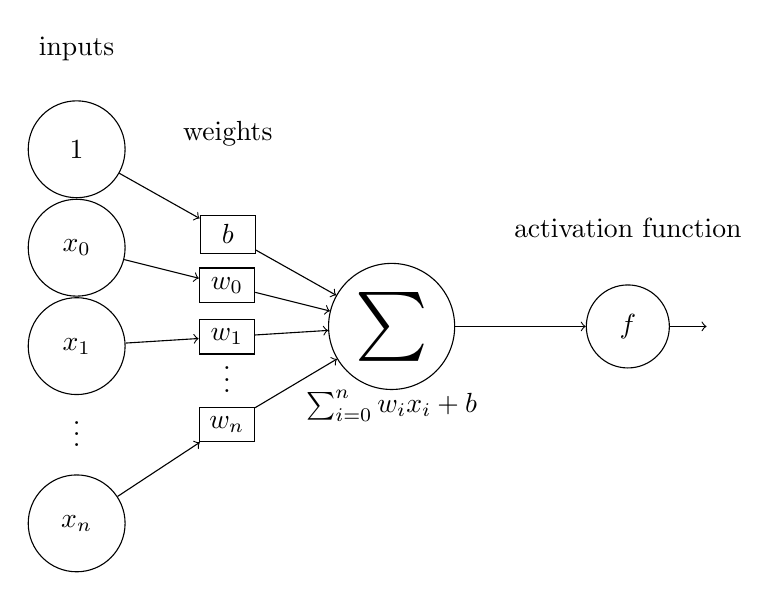
\begin{tikzpicture}
    % Draw input nodes
    \foreach \h [count=\hi ] in {$x_1$,$x_0$,$1$}{%
          \node[input] (f\hi) at (0,\hi*1.25cm-1.5 cm) {\h};
        }
    % Dot dot dot ... x_n
    \node[below=0.62cm] (idots) at (f1) {\vdots};
    \node[input, below=0.62cm] (last_input) at (idots) {$x_n$};
    % Draw summation node
    \node[functions] (sum) at (4,0) {\Huge$\sum$};
    \node[below=0.69cm] at (sum) {$\sum_{i=0}^n w_ix_i + b$};
    % Draw edges from input nodes to summation node
    \foreach \h [count=\hi ] in {$w_1$,$w_0$,$b$}{%
          \path (f\hi) -- node[weights] (w\hi) {\h} (sum);
          \draw[->] (f\hi) -- (w\hi);
          \draw[->] (w\hi) -- (sum);
        }
    % Dot dot dot ... w_n
    \node[below=0.05cm] (wdots) at (w1) {\vdots};
    \node[weights, below=0.45cm] (last_weight) at (wdots) {$w_n$};
    % Add edges for last node and last weight etc
    \path[draw,->] (last_input) -- (last_weight);
    \path[draw,->] (last_weight) -- (sum);
    % Draw node for activation function
    \node[functions] (activation) at (7,0) {$f$};
    % Place activation function in its node
    % \begin{scope}[xshift=7cm]
    %     \addaxes
    %     % flexible selection of activation function
    %     \relu
    %     % \stepfunc
    % \end{scope}
    % Connect sum to relu
    \draw[->] (sum) -- (activation);
    \draw[->] (activation) -- ++(1,0);
    % Labels
    \node[above=1cm]  at (f3) {inputs};
    \node[above=1cm] at (w3) {weights};
    \node[above=1cm] at (activation) {activation function};
\end{tikzpicture}

\captionof{figure}{A single Perceptron}
\label{fig:perceptron}

\end{center}
Neural networks are mostly build upon the Perceptron which can be thought of as the digital equivalent of a biological Neuron.
On a high level the Perceptron has a some number of numerical inputs and computes a singular output value based on that \cite{Rosenblatt58}.

A Perceptron is defined by its weights $w_i$, bias $b$ and the choice of the activation function $f$.
The bias is required so the Perceptron can output $y \neq 0$ when all $x_i = 0$.
Now having $n$ input values $x_0, x_1, ..., x_{n-1}, x_n$ the output of the perceptron can by computed like this:

$$
y=f\bigl(\sum_{i=0}^{n}w_i x_i + b\bigr)
$$


The figure \ref{fig:perceptron} shows such a perceptron.
A single basic Perceptron on its own is not particularly useful as
it only models linear decision boundaries and cannot learn the xor function \cite{MinskyPapert69}.

First we stack multiple Perceptrons to construct a layer. A layer has multiple
Perceptrons which calculate their output value with their own weights and biases on the same input values, which results
in as many output values as there are Perceptrons in the layer. Now one can construct a network which chains
multiple layers after each other, which results in a multilayer Perceptron (MLP), which is also known as a fully connected
feed forward network, as each layer is fully connected to the next layer in that each perceptron in layer $i$ 
is connected to each perceptron in layer $i+1$. The information strictly flows from input layer, through
intermediate hidden layers to the output layer, without any loops.
Mathematically a feed forward neural network, with $L$ layers and $0 < l \leq L$ can be described by

$$\mathbf{y}^{(l)} = f^{(l)}(\mathbf{W}^{(l)}\mathbf{y}^{(l-1)}+\mathbf{b}^{(l)})$$

where $\mathbf{W}^{(l)}$ represents the weight matrix of layer $l$, $\mathbf{b}^{(l)}$ the bias vector of layer $l$,
$\mathbf{y}^{(l-1)}$ the output vector of the previous layer or in case of $l=0$ the input vector
and $f^{(l)}$ is the activation function applied element-wise. \\


Now the choice of the activation function is very important, when using a multilayer Perceptron as when a linear activation function like the 
identity function is used for every Percetpron the entire network can be described in a single layer. Therefore
a non-linear activation function should be used to make the network capable of learning non-linear
decision boundaries. When choosing an activation function there are some important
properties which should be respected while making such a choice. The activation function should be fully differentiable, which makes
computing the gradient easier. It should also be computationally
cheap as its being run many times during a forward pass. \\

With loss functions the performance of a neural network on a given input can be computed by comparing the desired output with the 
predicted output of the model. Using loss functions we can quantify the error in the prediction of the neural network, which 
is a metric we can optimize for. There are again many options for choosing a loss function but it heavily depends on the nature of the
problem you're trying to solve by using a model: either classification or regression. A common loss function to use when trying to optimize 
regression tasks is the Mean Squared Error (MSE) \cite{Goodfellow16}:

$$\mathcal{L}(\mathbf{y},\mathbf{\hat{y}}) = \frac{1}{n}\sum^n_{i=1}{(y_i-\hat{y}_i)^2}$$

where $\mathbf{y}$ is the prediction of the model and $\mathbf{\hat{y}}$ the ground truth. When solving classification tasks the Cross Entropy Loss function is often used \cite{Goodfellow16}:


$$\mathcal{L}(\mathbf{y},\mathbf{\hat{y}}) = -\sum^n_{i=1}{y_i\log(\hat{y}_i)}$$

With loss functions we have a metric to optimize against, which can be used in an optimization algorithm called 
gradient descent. It will minimize the loss function by iteratively computing the error gradient and updating
the weights in the opposite direction of the gradient of the loss function. This is the update rule according
to gradient descent: \cite{Bottou10, Goodfellow16}

$$ \theta \leftarrow \theta - \eta \nabla_{\theta}\mathcal{L}(\theta)$$

Here, $\theta$ represents the parameters, $\eta$ the learning rate that determines the size of the step we take in 
the opposite direction of the gradient and $\nabla_{\theta}\mathcal{L}(\theta)$ denotes the gradient 
of the loss function with respect to parameters $\theta$. To compute the entire gradient, all the errors for the 
entire dataset would need to be averaged for the most accurate estimation of the gradient. Therefore variants 
like stochastic gradient descent exist, that first randomizes the order of dataset, second organizes it into batches of
the same size. Now we only average the gradient for all samples inside the batch and make an update to the model parameters \cite{Bottou10}.


To actually calculating the gradient the backpropagation algorithm is used. First we take out input data and do the
forward pass to compute the predictions. We can then calculate the loss by comparing the prediction to the desired result.
Now the idea behind backpropagation is to calculate the influence of the change weights and biases to the change in loss \cite{Rumelhart86}.
Mathematically this is represented by:


$$
\frac{\partial \mathcal{L}}{\partial \mathbf{W}^{(l)}} = \frac{\partial \mathcal{L}}{\partial \mathbf{y}^{(l)}} \frac{\partial \mathbf{y}^{(l)}}{\partial \mathbf{W}^{(l)}}
$$


where $\mathcal{L}$ denotes the loss, $\mathbf{W}^{(l)}$ represents the weight matrix at layer $l$ and $\mathbf{y}^{(l)}$ stands for the output matrix
for layer $l$. Now this can be calculated at the output layer $L$ to get the error signal for the layer $L-1$. 
Then the same computation can be applied to the layer $L-1$ to propagate the error back.

\subsection{Recurrent Neural Networks}

Classic feed forward neural networks are only able to handle fix sized data, because the size of the input layer
is fixed. Sequences of variable length, like timeseries, audio or language data require a different
architecture to still being able to compute the gradients properly. This can be achieved by recurrent
neural networks (RNNs). Recurrent neural networks accomplish that by carrying a hidden state across timesteps.

\begin{center}
  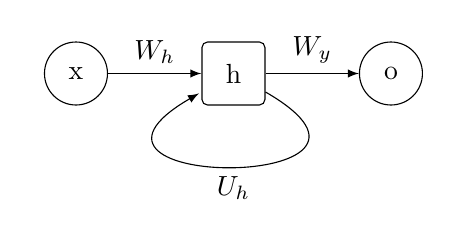
\begin{tikzpicture}[>=latex,
    % styles for clarity
    input/.style   ={draw, circle, minimum size=8mm},
    hidden/.style  ={draw, rectangle, rounded corners=2pt, minimum size=8mm},
    output/.style  ={draw, circle, minimum size=8mm},
    node distance = 2cm
  ]
    \node[input](x) at (0,0){x};
    \node[hidden](h) at (2,0) {h};
    \node[output](o) at (4, 0) {o};

    \draw[->] (x) -- node[above]{$W_h$} (h);
    \draw[->] (h) -- node[above]{$W_y$} (o);
    \path
      (h) edge[->,
            out=-30,
            in=-150,
            looseness=7,
            loop]
            node[below]{$U_h$}
      (h);
  \end{tikzpicture}
  \captionof{figure}{Simple RNN with one hidden layer} 
  \label{fig:rnn}
\end{center}

The RNN Cell is very similar to the Perceptron. It weights, biases and an activation function. Additionally 
it has a recurrent connection to itself: the output of a rnn cell at timestep $t$ is feed back to itself at timestep
$t+1$ multiplied by its own weight. That output value is called the hidden state $h_t$ of an rnn cell.
Figure \ref{fig:rnn} depicts a RNN cell with one hidden layer.
A Elman RNN is described by the forward state update and output projection \cite{Elman90}:

$$
h_t = \phi\!\bigl(W_h x_t + U_h h_{t-1} + b_h\bigr), \quad
y_t = \psi\!\bigl(W_y h_t + b_y\bigr).
$$
which can be understood as a neural network with fully connected input and output layers together with a hidden rnn layer.
The forward state update projection $h_t$ is similar to the perceptron where $b_h$ represents the bias, $W_h$ the weights,
with the addition of the term $U_hh_{t-1}$. $h_{t-1}$ is the hidden state of the last iteration and $U_h$ is the weight
matrix for the hidden state. Typically that output is then feed though a fully connected output layer map the
potentially high dimensional hidden state into the output space.\\


To calculate the gradient in a network with recurrent connections you need to unroll the network in time. The network
is unrolled over a sequence of length $T$, by creating $T$ copies of the same cell. All copies share the same weights.
The recurrent connections are now longer connected to themselves but their copy in the next copy. Unrolling converts 
the cyclic graph of a RNN into an acyclic graph, which is required for applying the standard backpropagation algorithm.
Figure~\ref{fig:rnn_unroll} depicts the unrolled network for $T=3$.

\begin{center}
  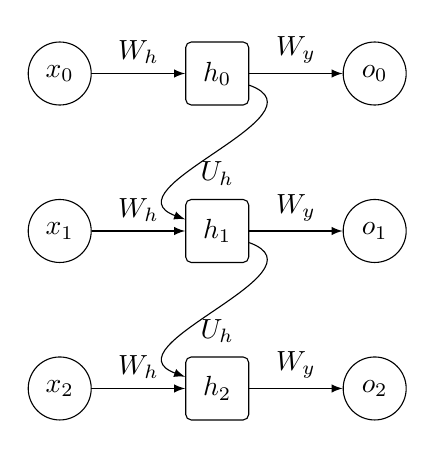
\begin{tikzpicture}[>=latex,
      % styles for clarity
      input/.style   ={draw, circle, minimum size=8mm},
      hidden/.style  ={draw, rectangle, rounded corners=2pt, minimum size=8mm},
      output/.style  ={draw, circle, minimum size=8mm},
      node distance = 2cm
    ]
    \foreach \t [count=\i from 1] in {0,1,2}{
      % place nodes at (0,-2*\i), (2,-2*\i), (4,-2*\i)
      \node[input]  (x\i) at (0,-2*\i) {$x_{\t}$};
      \node[hidden] (h\i) at (2,-2*\i) {$h_{\t}$};
      \node[output] (o\i) at (4,-2*\i) {$o_{\t}$};

      % input → hidden and hidden → output
      \draw[->] (x\i) -- node[above] {$W_h$} (h\i);
      \draw[->] (h\i) -- node[above] {$W_y$} (o\i);

      % hidden_{t–1} → hidden_t for t>0
      \ifnum\i>1
        \pgfmathtruncatemacro{\j}{\i-1}
        \draw[->, out=-20, in=160, looseness=1.5]
          (h\j) to node[below] {$U_h$} (h\i);
      \fi
    }
  \end{tikzpicture}
  \captionof{figure}{Unrolled Elman RNN for $T=3$.}\label{fig:rnn_unroll}
\end{center}


Applying backpropagation on an unrolled graph is called backpropagation through time (BPTT). On the acyclic graph 
the standard backpropagation algorithm can be applied, but the weights for all instances of the recurrent neural network
in the unrolled graph are shared. The final update for the parameter matrices are accumulated though time steps, so there 
is a contribution from everywhere a weight is used \cite{werb1990bptt}.


\subsection{Limitations of Recurrent Neural Networks}

Classic recurrent neural networks suffer from some limitations, which motivated the development 
of other RNN Variants notably LSTM networks.

\begin{enumerate}[label=(\roman*)]
\item \textbf{Vanishing and exploding gradients.}  During BPTT the gradient with respect to earlier timesteps involves products of Jacobian
  matrices $\partial h_t/\partial h_{t-1}$.  For many activation functions this product tends to shrink or blow up exponentially with
  the number of timesteps, causing the gradient norm to \emph{vanish} or \emph{explode}.
  As a consequence the network either fails to learn long‑range dependencies or becomes numerically unstable~\cite{hochreiter1997lstm,pascanu2013rnntraining}.
  Exploding gradients can be taken care of by clipping the gradient to a maximum value \cite{pascanu2013rnntraining}.
  Vanish gradients though cannot be mitigated this easily. The vanishing gradients problem is the main motivation behind the
  development of LSTM networks.
\item \textbf{Limited memory capacity.}  The entire past of the sequence must be compressed into a single hidden vector $h_t$.
  In practice the dimensionality of $h_t$ is bounded by computational constraints, creating a tight information bottleneck.
  Empirical analyses show that standard RNNs spontaneously forget information that is not constantly reinforced.
\item \textbf{Difficulty modelling very long sequences.}  Even when exploding gradients are clipped and vanishing 
  gradients mitigated, the truncation window in BPTT means the effective context length is often limited to a few hundred
  time steps.  Tasks such as document‑level language modelling require mechanisms that can propagate information across thousands of steps \cite{pascanu2013rnntraining}.
\item \textbf{Bias towards recent inputs.}  The recurrent update $h_t=\phi(W_h x_t + U_h h_{t-1})$ blends the new input with a 
  transformed version of the previous hidden state.  Without gating, this blend is rigid and the network cannot dynamically decide 
  to \emph{copy} or \emph{forget} information.  As a result, RNNs tend to over‑weight recent inputs and under‑weight older ones.
\end{enumerate}

\section{LSTM Architecture (Fynn)}

This section focuses on the principle of operation of LSTMs, first providing an intuitive overview of how they work. Next, the most common LSTM network topology is covered, followed by an examination of both the original and modern mathematical formalization of the architecture.

\subsection{Principle of Operation (Fynn)}
This section first introduces some of the building blocks that comprise the LSTM architecture, such as the constant error carousel and gate units. It then explains how the architecture is constructed and operates.

\subsubsection{Constant Error Carousel (Fynn)}
For a single neuron $j$, it is possible to achieve constant error flow over time by setting the weight of its feedback connection $w_{jj}=1$ to 1 and selecting the linear activation function $f_j(x)=x\ \forall x$. This construction, shown in Figure \ref{fig:CEC}, is called a Constant Error Carousel (CEC).\cite{hochreiter1997lstm}
\begin{center}
\begin{tikzpicture}
\node[circle,draw] (unit_j) {$f_j(x)=x$};
\draw[->] (unit_j) edge[loop above] node {$w_{jj}=1$} (unit_j);
\draw[->] (-3,0) -- node[above] {$w_{ji}$} (unit_j.west);
\draw[->] (unit_j.east) -- node[above] {$w_{jk}$} (3,0);
\end{tikzpicture}
\captionof{figure}{Single Neuron Constant Error Carousel\\Source: Based on \cite{hochreiter1997lstm}} 
\label{fig:CEC}
\end{center}
This works because the error backflow is scaled by  $f'_j(net_j(t))w_{jj}$ (where $net_j(t)$ is the activation of neuron $j$ at time $t$) at every time step. This is why ensuring this expression remains fixed at 1 mitigates exploding and vanishing gradients. Since $f'(x)=1$, this is the case for the chosen activation function and weight.\cite{hochreiter1997lstm} \\
While this theoretically solves the problem of exploding and vanishing gradients in recurrent neural networks, it introduces new issues in practice, rendering the solution impractical without further modifications. Consider another neuron, $i$, with an activation, $y^i(t)$, that is connected to neuron $j$ with a weight, $w_{ji}.$  For each time step, the activation of $j$ at the previous time step is added to $y^i(t)w_{ji}$. This makes the CEC a type of memory that stores previous inputs by adding them together.\cite{hochreiter1997lstm} \\
However, as $w_{ji}$ is the only factor determining whether the activations of $i$ are stored in memory, it often receives conflicting weight update signals during training, resulting in unstable training. Similarly, the output from the CEC's memory to another neuron $k$ is controlled by a single weight, $w_{jk}$, which also leads to unstable training. Furthermore, storing and retrieving the memory of $j$ often depends on the context; therefore, a context-sensitive mechanism is needed to control access to the CEC's memory.\cite{hochreiter1997lstm}

\subsubsection{Gate Units (Fynn)}

Hochreiter and Schmidhuber proposed a solution to this problem in the form of the so-called 'gate unit'.\cite{hochreiter1991}\\
Gate units allow the flow of information to and from a neuron to be restricted based on the context.
They work by scaling an input by multiplying it by a number computed from the context. This scaling factor is computed in the same way as for a regular neuron, where inputs from other neurons are added together to form a weighted sum, which is then passed through an activation function..\cite{hochreiter1997lstm}

\subsubsection{Memory Cell (Fynn)}
Combining a Gate Unit with the input and output of a CEC, along with the scaling functions $g$ and $h$, results in a structure known as a Memory Cell or LSTM Cell, as illustrated in Figure \ref{fig:lstm-cell}. These cells are the building blocks of LSTM networks and replace conventional neurons.\cite{hochreiter1997lstm} \\
The gate unit on the input side of the cell is often referred to as the 'input gate' or 'update gate', while the gate on the output side is known as the 'output gate'.\cite{hochreiter1997lstm} \\
\begin{figure}[h!]
    \centering
    \includegraphics[width=\linewidth]{LSTM-Cell-Diagram.png}
    \caption{LSTM Cell\\ Source: \cite{hochreiter1997lstm}}
    \label{fig:lstm-cell}
\end{figure}

The circles in Figure \ref{fig:lstm-cell} represent neurons. The arrows pointing into them represent scaled inputs, and the black dots represent multiplication.\cite{hochreiter1997lstm} \\
The arrows pointing into the cell from the bottom represent the inputs for the gate units.
The arrows pointing into the cell from the bottom in Figure \ref{fig:lstm-cell} represent the inputs for the gate units. For each gate, all inputs are scaled by their respective weights and summed together. The result is then passed through an activation function to obtain the gate activations, $y^{in_j}$ and $y^{out_j}$, which control access to the cell's memory.\cite{hochreiter1997lstm} \\
In Figure \ref{fig:lstm-cell}, the cell's input, $net_{c_j}$, is computed in the same way as for the gate units by summing the weighted inputs. This input is then scaled first by the function $g$ and then by the input gate's activation $y^{in_j}$ , after which it reaches the cell's internal CEC. \cite{hochreiter1997lstm} \\
Here, the new input is added to the previous CEC activation to update the cell's internal memory, also known as its internal state.\cite{hochreiter1997lstm} \\
Finally, to generate an output from the cell's memory, the internal CEC output is first scaled by a function $h$ and then scaled again by the output gate activation $y^{out_j}$, in the same way as for the input gate. This results in the cell output activation, $y^{c_j}$.\cite{hochreiter1997lstm} 

\subsection{Network Topology (Fynn)}

In Hochreiter and Schmidhuber's paper, the specific inputs for the cells and gates are not defined, as these depend on the chosen network topology. These inputs could be the outputs of input units, memory cells, gate units, or conventional hidden units.\cite{hochreiter1997lstm}\\
The most commonly used implementations of the LSTM architecture, such as those included in machine learning libraries like PyTorch and TensorFlow, connect all the outputs of each cell to all the inputs and gate inputs of each cell, as well as to each cell's biases. They also connect other inputs that do not depend on the state of the cells to all inputs and gate inputs of each cell.\cite{smagulova2019notation, keras-lstm, real-pytorch-lstm, pytorch-lstm}

\subsection{Mathematical Formalization (Fynn)}

This section focuses on two formalisation methods for the architecture. The first is the original formalisation by Hochreiter and Schmidhuber. The second is a modern matrix formulation for the most commonly used network topology.

\subsubsection{Single Memory Cell (Fynn)}
For a single memory cell $c_j$ the cell net input can be defined as:\cite{hochreiter1997lstm}
$$net_{c_j}(t)=\sum_u w_{c_ju}y^u (t-1)$$
The input gate net input as:\cite{hochreiter1997lstm}
$$net_{in_j}(t)=\sum_u w_{in_j u}y^u(t-1)$$
And the output gate net input as:\cite{hochreiter1997lstm}
$$net_{out_j}(t)=\sum_uw_{out_j u}y^u(t-1)$$
The summation index $u$ represents any units connected to the cell and its values depend on the networks topology.\cite{hochreiter1997lstm} \\
The are the result of passing the gate net inputs through their respective activation functions $f_{in_j}$ and $f_{out_j}$:\cite{hochreiter1991}
$$y^{in_j}(t)=f_{in_j}\left(net_{in_j}(t)\right)$$
and
$$y^{out_j}(t)=f_{out_j}\left(net_{out_j}(t)\right)$$
As the internal state always adds the new input scaled by the input gate to the previous state it can be defined as:\cite{hochreiter1997lstm}
$$s_{c_j}(0)=0$$
and
$$s_{c_j}(t)=s_{c_j}(t-1)+y_{in_j}(t)g\left(net_{c_j}(t)\right)\ \text{ for } t>0$$
Using this, the cells output can be calculated by scaling the cell state using the output gate activation:\cite{hochreiter1997lstm}
$$y^{c_j}(t)=y^{out_j}(t)h\left(s_{c_j}(t)\right)$$
\subsubsection{Block of Memory Cells (Fynn)}
For the most commonly implemented network topology, in which the cell outputs are fully connected to their inputs and gate inputs, as well as to some additional inputs which are also fully connected to the cell inputs and gate inputs and to all inputs, each of which has a bias, the block can be described using matrix notation:\cite{smagulova2019notation}
\\
The activation of all input gates can be described by:\cite{smagulova2019notation}
$$i_t=\sigma\left(W^{(i)}x_t+U^{(i)}h_{t-1}+b^{(i)}\right)$$
Similarly the output gates activations are defined by:\cite{smagulova2019notation}
$$o_t=\sigma\left(W^{(o)}x_t+U^{(o)}h_{t-1}+b^{(o)}\right)$$
And the inputs of the cells, defined by:\cite{smagulova2019notation}
$$g_t=g\left(W^{(g)}x_t+U^{(g)}h_{t-1}+b^{(g)}\right)$$
The state for all cells can be described by:\cite{smagulova2019notation, hochreiter1991lstm}
$$C_t=g_t\odot i_t+C_{t-1}$$
From this the outputs of the cells can be defined as:\cite{smagulova2019notation, hochreiter1997lstm}
$$h_t=o_t\odot h(C_t)$$
The $\odot$ Operator is called the Hadamard product, which is defined as component wise multiplication of two vectors, which allows each cells input and output to be gated individually.\cite{gokmen2018hadamard, smagulova2019notation} \\ 

The function $\sigma$ (or $f$  is the sigmoid function defined as: \cite{hochreiter1997lstm} $$\sigma(x)=\frac{1}{1+\exp(-x)}$$
For the experiments in the original papers the functions $g$ and $h$ were defined as:\cite{hochreiter1997lstm}
$$g(x)=\frac{4}{1+\exp(-x)}-2$$
and \cite{hochreiter1997lstm}
$$h(x)=\frac{2}{1+\exp(-x)}-1$$
Today the $\tanh$ function is commonly used for the functions $g$ and $h$.\cite{smagulova2019notation}

\subsection{Results (Fynn)}

In their 1997 paper, Schmidhuber and Hochreiter compared the LSTM architecture with other architectures for sequential data. These included standard recurrent neural networks (RNNs), which were trained using either back propagation through time (BPTT) or real-time recurrent learning (RTRL); Elman networks, which were trained using Elman's procedure; recurrent cascade-correlation; and neural sequencing chunking.\cite{hochreiter1997lstm}  \\

In their first experiment, they trained their networks using an embedded reber grammar. As Figure \ref{fig:exp1res} shows, while BPTT and RTRL did not always learn the grammar, the LSTM architecture always managed to learn the task. Furthermore, it learned the task much faster than the other architectures.\cite{hochreiter1997lstm}
\begin{figure}
    \centering
    \includegraphics[width=0.75\linewidth]{ResultsTask1.png}
    \caption{Results of training the models on sequences with different time lags are shown, along with the percentage of successful trials and the number of training examples presented to the model until it learned the task. This table compares the following architectures: Real Time Recurrent Learning (RTRL), Back Propagation Through Time (BPTT) and Neural Sequence Chunking (CH). \\ Source: Taken from \cite{hochreiter1997lstm}}
    \label{fig:exp1res}
\end{figure}

The different architectures were also tested using noisy and noiseless sequences with a long time lag.
For these inputs, one-hot encoding was used to encode the symbols.\cite{hochreiter1997lstm, qiu2022onehot}
\\ For noise-free sequences, the models were trained on two similar sequences: one in the form of $(x, a_1, ..., a_n, x)$, and the other in the form of $(y, a_1, ..., a_n, y)$. This means that the model must store the first token for $n$ time steps in order to correctly predict the final token of the sequence.\cite{hochreiter1997lstm}\\
\begin{figure}[h!]
    \centering
    \includegraphics[width=0.75\linewidth]{restask2.png}
    \caption{Results of training the models on sequences with different time lags, showing the percent of successful trials as well as the number of training examples till presented to the model until it learned the task. The architectures compared in this table are Real Time Recurrent Learning (RTRL), Back Propagation Through Time (BPTT) and neural sequence chunking (CH). \\Source: Taken from \cite{hochreiter1997lstm}}
    \label{fig:exp2res}
\end{figure}
As shown in Figure \ref{fig:exp2res}, for short time lags such as $n=4$ , both RTRL and BPTT can learn the task in some runs. However, for $n=10$, they always fail. Neural sequence chunking was able to learn the task in some runs, even with time lags as large as $n=100$. The LSTM architecture learned the task every time and did so much faster than the other methods.\cite{hochreiter1997lstm}\\

As the chunker sometimes learned to predict local regularities in the sequence in this experiment, another experiment was run where the sequence of length $n$, $(a_1, ..., a_n)$, was replaced by a random sequence of the same length. The RTRL, BPTT and chunker models all failed to learn the task, whereas the LSTM model was able to learn it every time.\cite{hochreiter1997lstm}\\
\\
Another test involved classifying sequences containing noise. For this, sequences were generated where only the first N elements contained information, while the rest were noise. Another test involved adding noise to data that contained information. In both cases, the LSTM architecture was able to learn the task at hand.\cite{hochreiter1997lstm}
\\
The LSTM architecture was also able to solve the addition problem.\cite{hochreiter1997lstm}\\
Here, a sequence consists of a pair of numbers, where the first number is a real number between $-1.0$ and $1.0$, and the second number is $1.0$, $0.0$, or $-1.0$. The objective is to calculate the sum of the first number in each pair for which the second number is $1.0$. As with the previous problem, the LSTM architecture was able to learn the task and correctly process most of the test sequences.\cite{hochreiter1997lstm}\\
In a similar task where the network had to multiply two marked numbers, the LSTM architecture was once again able to learn the task. \cite{hochreiter1997lstm}
\section{Limitations and Alternatives (Fynn)}

This section will first review some of the limitations of LSTM networks. Afterwards, variations of the architecture that attempt to address these issues will be discussed. Finally, the LSTM architecture will be compared to the Transformer architecture, which has replaced LSTMs in many applications.

\subsection{Limitations (Fynn)}
Although LSTMs solve some of the problems associated with classical RNNs, they also have some disadvantages, including:
\begin{itemize}
    \item \textbf{Computational Intensity:} Computational intensity: As an LSTM cell requires additional weights for the gates, the number of weights can increase by up to a factor of \begin{math} 9 \end{math}. However, this is usually not a significant issue, as LSTM networks typically have a similar number of weights to other RNNs.\cite{hochreiter1997lstm}\\ However, in applications that require low power, such as mobile devices, this could cause problems. \cite{rizakisFPGAlstm}
    \item \textbf{Exploding Gradients:} Although the LSTM architecture mitigates the issue of vanishing gradients, it does not eliminate that of exploding gradients.\cite{pascanu2013rnntraining} This can be achieved using alternative techniques, such as gradient clipping.\cite{gradient-clipping, pascanu2013rnntraining}
    \item \textbf{Limited GPU utilization and memory bottlenecks:} LSTM networks do not utilize the GPU fully, as they are sequential in nature and can't be easily parallelized, which makes training less efficiently on modern GPUs. Furthermore, they are often limited by the available GPU memory.\cite{zheng2018scalability, zheng2020scalability}  
    \item \textbf{Worse performance on less complex sequences:} Although LSTMs perform better than some other architectures, such as GRUs, on sequences with high complexity, they struggle more on simpler sequences.\cite{cahuantzi2023lstmvsgru} 
    \item \textbf{Worse performance on short sequences:} LSTMs tend to perform poorly with short sequences, often having significantly higher losses. \cite{bolboaca2023lstmperformance} 
        \item \textbf{Over fitting:} Especially when trained on small data sets, LSTMs tend to over fit, which results from the large amount of parameters in a model. \cite{kinoyama2021overfitting}
        \item \textbf{Sensitivity to Hyper Parameters:} The performance of LSTM Networks can be significantly affected by hyper parameters, such as the batch size or learning rate. Selecting the right hyper parameters so that an LSTM Network works efficiently can require loads of trial and error. \cite{hochreiter1997lstm}
        \item \textbf{Interpretability:} The method with which LSTM Networks make their prediction is hard to interpret. This limits the extend to which LSTM Networks can be used in industries where explainable models are needed. \cite{firouzjaee2024interpret}
\end{itemize}

\subsection{Variants (Fynn)}

Many variations of the LSTM architecture have been developed to address some of its limitations. This section will provide an overview of some of the most important variations, such as the addition of a forget gate or bidirectional LSTMs.

\subsubsection{LSTM with Forget Gate (Fynn)}
\begin{figure}[h!]
    \centering
    \includegraphics[width=0.75\linewidth]{Structure-of-LSTM-cell-which-introduces-three-special-gates-Input-Gate-i-Forget-Gate.png}
    \caption{LSTM Cell with forget gate\\ Source: \cite{nguyen2022lstmforgetgraphic}}
    \label{fig:lstm-forget}
\end{figure}
One of the first variation of Hochreiter and Schmidhuber's architecture, was the introduction of a forget gate. The reason for its introduction is that there is no way for the internal state of the cell to be reset in the original architecture. To fix this a forget gate can be introduced, which restricts how much of the previous state is kept in the next time step.\cite{gers1999forgetgate}\\
Figure \ref{fig:lstm-forget} shows an LSTM cell, with the added forget gate on the left of the cell. Note that the input gate is labeled as "Update Gate" in this graphic.\\
The forget gate is implemented like the other with\cite{gers1999forgetgate}
\begin{equation}
    net_\varphi(t)=\sum_uw_{\varphi\ u}y^u(t-1)
    \label{eqn:forget-net-in}
\end{equation}
and
\begin{equation}
    y^\varphi(t)=f_\varphi\left(net_\varphi(t)\right).
    \label{eqn:forget-actiavtions}
\end{equation} 
Equation \ref{eqn:forget-net-in} describes the net inputs for the forget gate, and equation \ref{eqn:forget-actiavtions} describes the activation for the forget gate. Using those a new equation for the cell state can be defined as\cite{gers1999forgetgate}
\begin{equation}
    s_c(t)=y^\varphi(t)s_c(t-1)+y^{in}(t)g\left(net_c(t)\right).    
\end{equation}
The forget gate can also be defined using the matrix notation, where its activations are given by:\cite{smagulova2019notation}
$$f_t=\sigma\left(W^{(f)}x_t+U^{(f)}h_{t-1}+b^{(f)}\right)$$
and the internal state's of the cells can be defined as:\cite{smagulova2019notation}
$$C_t=g_t\odot i_t+f_t\odot C_{t-1}$$

The addition of a forget gate is very common, and many implementations of LSTMs in popular machine learning frameworks include one.\cite{smagulova2019notation,keras-lstm, real-pytorch-lstm, pytorch-lstm} 

\subsubsection{Bidirectional LSTM (Leon)}

\begin{figure}[h!]
    \centering
    \includegraphics[height=7.5cm]{brnn.png}
    \caption{Unrolled bidirectional recurrent network\\ Source: \cite{graves2013speechrecognitiondeeprecurrent}}
    \label{fig:brnn}
\end{figure}

Building upon bidirectional RNN \cite{Schuster97} the bidirectional LSTM processes input sequences not only in the 
forward direction but also in the backward direction. It has 2 lstm layers where one is processing the forward direction
and the other the backward direction. The final representation consists of the outputs of the 2 layers which are then merged together,
usually concatenation is used. In the final encoding both information about the past and the future are embedded \cite{Graves05}.\\
Figure \ref{fig:brnn} shows a bidirectional rnn with 2 recurrent layers. The first layer $\overrightarrow{h}_t$ processes
the input in the forward direction while the second layer $\overleftarrow{h}_t$ in the backward direction.



This architecture is used in sequence labeling \cite{huang2015bidirectionallstmcrfmodelssequence} and speech recognition \cite{graves2013speechrecognitiondeeprecurrent}.

\subsection{LSTM vs Transformers (Leon)}

The Transformer architecture relies on the attention mechanism as introduced in “Attention Is All You Need” paper.
The main difference is that the recurrent update used by LSTM networks is replaced by a self-attention mechanism \cite{vaswani2017attention}.\\


First, each input sequence is mapped to learned token embeddings and positional encodings. Positional encoding 
inject order information about where a token is inside of a sequence of tokens inside its token representation instead of in the architecture of the model as in RNNs.


The next innovation sparked by transformers was self-attention. Self-attention lets the model assign learned weights to the influence of every token on every other token.
When predicting the next token in sequence some tokens capture more semantic meaning than others and theise will be highlighted for the neural network by the 
attention mechanism. The attention is learned by the transformer in the training process \cite{vaswani2017attention}.
The computational and memory cost of self-attention as presentend in \cite{vaswani2017attention} is $\mathcal{O}(n^2)$. Though there are efforts
to optimize the self attention mechanism to reduce its complexity to $\mathcal{O}(n)$. \cite{katharopoulos2020transformersrnnsfastautoregressive}


While LSTM networks propagate past information by passsing the hidden state into the next iteration, transformers attend to the entire input sequence in every
step. Transformers do not suffer from vanishing or exploding gradient issues like RNN do.


Because self-attention removes any timestep-to-timestep dependency, a Transformer can process all tokens in a sequence simultaneously. 
In the original paper, Vaswani et al. report training their English-German “base” model to state-of-the-art quality in roughly 
12 hours on 8 P100 GPUs—several-times faster than earlier RNN/LSTM systems that must handle tokens one-by-one \cite{vaswani2017attention}.


Both architectures have their own advantages and disadvantages. LSTM networks are great at handling sequential data and 
remembering long term dependencies. Transformers are best at processing the data in parallel.


\section{Applications (Fynn)}

LSTM Networks have been used for a variety of applications through out the years.\\
This Section will highlight some of the most important applications of LSTM Networks, and provide some specific examples of how LSTMs where used in those areas.

\subsection{Speech Recognition (Leon)}

We have already established that LSTM networks are great at working with sequence data. One example where LSTM networks
have been successfully used is speech recognition \cite{Graves04}. The LSTM network learns temporal patterns in audio and captures long 
term relationships. They have achieved state of the art results in a paper by Google in 2014 \cite{sak2014longshorttermmemorybased}.
Researchers at google showed that a deep LSTM network outperformed traditional deep neural networks for this problem.
It was even better then a feed forward neural network with 10x more parameters \cite{sak2014longshorttermmemorybased}.\\


They used an LSTM variant called Long Short-Term Memory Projected (LSTMP) architecture \cite{sak2014longshorttermmemorybased} which
outperformed the traditional LSTM architecture. The LSTMP architecture differs from the traditional LSTM one by not having a LSTM layer
which output is directly connected to its input but they first do a linear projection with a fully connected layer and its output will represent the 
hidden state of the cell.

\subsection{Time Series Forecasting (Fynn)}
While LSTMs can be used to forecast time series, they often are inferior to other methods.\cite{gers2001timeseries} But for certain applications, like speech or music, they are a better choice, as they perform better on more complex sequences.\cite{gers2001timeseries, cahuantzi2023lstmvsgru}\\
In a 2022 article by Torres, they use an deep LSTM network, to predict electricity demands and achieve errors of just \begin{math}1.5\%\end{math}.\cite{torres2022elctricityforecasting}\\
Kılıç et al. (2024) uses the LSTM architecture to predict electricity prices, and achieve better results compared to other architectures.\cite{nielsen2024electricitypriceforcasting}

\subsection{Music and Audio (Fynn)}
Music has structures and patterns, where the next note or chord depends on the previous ones. LSTMs can learn those patterns and predict what comes next, which allows them to generate music.\cite{eck2002musicgeneration}\\
In their 2002 paper Eck and Schmidhuber use an LSTM network to generate chord progressions, as well as melodies and chord progressions. Their network successfully managed to pick up on patterns in a style of music and reproduce those patterns to compose new music in the same style.\cite{eck2002musicgeneration}  

\subsection{Medical (Leon)}

A 7 layer LSTM network was trained to detect Type 2 diabetes in the early stages in Oman. The model is composed of five stacked
LSTM layeres with 20 Units each feeding into a fully connected output layer. It reaches \begin{math}99.4 \%\end{math} accuracy and an 
AUROC of \begin{math}0.945\end{math} while maintaining \begin{math}100 \%\end{math} sensitivity on a \begin{math}20 \%\end{math} hold-out set \cite{AlSadi2024LSTM}.
These results surpass the logistic regression baseline.


\section{Conclusion (Fynn)}
The LSTM architecture introduced gate units and memory cells, effectively eliminating the vanishing gradient problem that had prevented RNNs from reaching their full potential.\cite{hochreiter1997lstm} 
This enabled LSTMs to be used for tasks such as time series forecasting, music generation, and natural language processing.\cite{eck2002musicgeneration,nielsen2024electricitypriceforcasting,gers2001timeseries,torres2022elctricityforecasting,sak2014longshorttermmemorybased}\\
Although LSTMs have been replaced by architectures such as transformers in many applications, they are still useful because they perform better with small datasets. This is why further research into improving the performance of this architecture is likely.\cite{alselwi2024lstmfuture} Furthermore, they will likely form the basis of new architectures. For example, LSTM-Transformer hybrid architectures already exist today. \cite{zhao2025lstmtransformerhybrid} 

\appendix

\section{Implementation (Fynn)}

The following code is an implementation of the original LSTM Architecture as described in the original paper by Hochreiter and Schmidhuber using PyTorch. It takes inspiration from the keras implementation of the LSTM architecture and the implementation from a blog post on medium by the user "noplaxochia", but it leaves out the forget gate.

\begin{lstlisting}
import torch

class LSTMCell(torch.nn.Module):
    
    size : int # Input Size (1D)
    
    w_i_c : torch.Tensor # Input gate weights
    w_i_x : torch.Tensor # Input gate weights
    w_c_c : torch.Tensor # Cell gate weights
    w_c_x : torch.Tensor # Cell gate weights
    w_o_c : torch.Tensor # Output gate weights
    w_o_x : torch.Tensor # Output gate weights
    
    b_i : torch.Tensor # Input gate biases
    b_c : torch.Tensor # Cell gate biases
    b_o : torch.Tensor # Output gate biases
    
    def __init__(self, size : int):
        super(LSTMCell, self).__init__()
        self.size = size

        # Initialize weights and biases        
        self.w_i_c = torch.nn.Parameter(torch.randn(size, size) * 0.01)
        self.w_i_x = torch.nn.Parameter(torch.randn(size, size) * 0.01)
        self.w_c_c = torch.nn.Parameter(torch.randn(size, size) * 0.01)
        self.w_c_x = torch.nn.Parameter(torch.randn(size, size) * 0.01)
        self.w_o_c = torch.nn.Parameter(torch.randn(size, size) * 0.01)
        self.w_o_x = torch.nn.Parameter(torch.randn(size, size) * 0.01)
        
        self.b_i = torch.nn.Parameter(torch.zeros(size))
        self.b_c = torch.nn.Parameter(torch.zeros(size))
        self.b_o = torch.nn.Parameter(torch.zeros(size))    
        
    @staticmethod
    def _f(x: torch.Tensor) -> torch.Tensor:
        """Gate unit logistic sigmoid with range [0, 1]."""
        return torch.sigmoid(x)
    
    @staticmethod
    def _g(x: torch.Tensor) -> torch.Tensor:
        """Function g with range [-2, 2]."""
        return torch.sigmoid(x) * 4 - torch.ones_like(x) * 2
    
    @staticmethod
    def _h(x: torch.Tensor) -> torch.Tensor:
        """Function h with range [-1, 1]."""
        return torch.sigmoid(x) * 2 - torch.ones_like(x)
    
    def forward(self, x_t : torch.Tensor, y_tm1 : torch.Tensor, c_tm1 : torch.Tensor) -> tuple[torch.Tensor, torch.Tensor]:
        # Ensure x_t is the right shape for matrix multiplication
        if x_t.dim() == 0:  # scalar
            x_t = x_t.unsqueeze(0)
        
        #Input gate
        net_i = self.w_i_c @ y_tm1 + self.w_i_x @ x_t + self.b_i
        i_t   = self._f(net_i)
        
        # Output gate
        net_o = self.w_o_c @ y_tm1 + self.w_o_x @ x_t + self.b_o
        o_t   = self._f(net_o)
        
        # Cell gate & Update Cell state
        # Compute cell gate
        net_c = self.w_c_c @ y_tm1 + self.w_c_x @ x_t + self.b_c
        c_t = c_tm1 + i_t * self._g(net_c) # Update cell state
        y_t = o_t * self._h(c_t)           # Compute output
        
        return y_t, c_t
\end{lstlisting}

\bibliographystyle{alpha}
\bibliography{abbrev,seminar_report}
\end{document}
